
%********** Chapter 6 **********
\chapter{Generic Board Game}\index{Generic Board Game}\index{projects!Generic Board Game}\label{ch:boardgame}

\section{Introduction}

This chapter introduces the fourth project: a generic board game.  In this game, two players roll a simulated die to move along a board trying to get to the goal.  Along the way, they land on squares that may either move them backwards or forwards.  The game has the same general format as  Candyland{\texttrademark}, Chutes (or Snakes) and Ladders{\texttrademark}, Life{\texttrademark}, and similar board games.  Like the earlier projects, the initial version of the program is generic, just the general framework for a board game, but it is designed to be easy to modify to meet the programmer's needs and interests.

This project reviews the topics from the earlier chapters, particularly classes, scope, and files, and introduces several new topics:
\begin{tight_itemize}
\item Pass-by-reference\index{pass-by-reference}\index{arguments!pass-by-reference}
  \item Arrays\index{arrays}
  \item Characters (the \cf{char} type)\index{characters}\index{char@{\cf{char}}}\index{type!char@{\cf{char}}}
  \item Global variables\index{globals}
   \item Constants\index{constants}
\end{tight_itemize}

 Pass-by-reference is an alternative method of passing arguments to functions, it allows changes made to the function's parameters to persist in the calling function.  Arrays are data structures that store multiple data of the same type; for example, a list of integers or doubles or objects of the same type.  They are one of the most widely used, and useful, of the basic data structures.  Characters, abbreviated \codefont{char} in code, are a new type that stores a single character: `a', `b', `=', `5', etc.  Global variables are variables whose scope extends throughout the entire program.   Constants are named boxes that store values that cannot change.

\section{The Program}

Listings~\ref{listing:GenericGameA},~\ref{listing:GenericGameB}, and~\ref{listing:GenericGameC} present the code for the board game.  In addition, this program requires data, which is read from a file.  Listing~\ref{listing:game.txt} presents the initial data file.  


To compile and run the program, enter the code from Listings~\ref{listing:GenericGameA},~\ref{listing:GenericGameB}, and~\ref{listing:GenericGameC} (but not Listing~\ref{listing:game.txt}) in that order into a single program\ (do \emph{not} enter the line numbers).  Try to figure out what the statements do.  Many of them should be very familiar by now, but others will be new.

\begin{minipage}{\textwidth}
\begin{lstlisting}[language=C++,numbers = left,xleftmargin=4.0ex, basicstyle=\small, emph={move,message,symbol,board_length},emphstyle = \color{\mycolor}, 
showstringspaces=false,
caption = {Initial code for the Generic Board Game program, including the include statements, declaration of the \cf{square class}, prototypes for the other functions defined as part of the program, and a global constant called \codefont{board\_length}.},
label={listing:GenericGameA}]
 #include<iostream>
 #include<string>
 #include<fstream>
 #include<ctime>
 #include<cstdlib>
 using namespace std;
                            // Declaration of the square class
class square{
  private:
     int move;
    string message;
    char symbol;
  public:
    square();
    void print();
    int action();
    void set(int,char,string);
};
                            // Function Prototypes
void print_board(square[], int, int);
void read_board(square[]);
void check_position(int &);
                           // Global variables
const int board_length = 20;
\end{lstlisting}
\end{minipage}

Next, create a plain text file called ``game.txt'' containing the text from Listing~\ref{listing:game.txt}.  This file should be in the same directory or folder as the program file.

Once the entire program has been entered and the data file ``game.txt'' has been created, compile the program.  As always there may be some copying errors that need to be fixed.  Once the program compiles, run it.  Try to figure out what the data file is used for.

As with the other projects in the text this program has some shortcomings.  Most notably it is, as advertised, a generic game.  However, the program is written to make it very easy to customize.  Instead of game with generic messages like ``Go back 2 squares'' it can be turned into a specific game. For example, a sailing game with messages like ``Strong currents push your ship backwards'' or ``Good winds advance 2 squares.''  As explained later in the chapter, giving the game a specific theme only requires changing the file ``game.txt.'' 

\subsection{Pass-by-reference}\index{pass-by-reference}\index{arguments!pass-by-reference}\index{functions!pass-by-reference}

Functions, arguments, and parameters were introduced in Chapter 3.  ``Standard'' function parameters are pass-by-value: the value of the arguments are copied into the function.  An alternative approach is \emph{pass-by-reference}.  In pass-by-reference, a \emph{reference} to the ``box'' holding the argument is passed to the function rather than the argument's \emph{value}.\footnote{The reference is actually the \emph{address} in memory where the argument is stored.  Because the function receives the address in memory of the variable it can change the value directly.  Addresses and memory are discussed in more detail in Chapter 7.} This means that the function has direct access to the ``box'' holding the argument value in the calling function.   Figure~\ref{fig:passbyrefarguments} illustrates this idea.  Any changes that the function makes to an argument persists after the function exits, even if the new value is not returned by the function.  

\begin{minipage}{\textwidth}
\renewcommand*\thelstnumber{\the\value{lstnumber}b}
\begin{lstlisting}[language=C++,numbers = left,xleftmargin=4.0ex, basicstyle=\small, emph={current_player,player1_position,player2_position,the_board},emphstyle = \color{\mycolor},
showstringspaces=false,breaklines=true,
  breakatwhitespace=true,
caption = {The \codefont{main()} function for the Generic Board Game.},
label={listing:GenericGameB}]
int main(){
  int current_player = 1, roll;
  int player1_position = 0, player2_position = 0;
  square the_board[board_length];  // declare an array of squares
  srand(time(NULL));
  read_board(the_board);
  print_board(the_board,player1_position,1);
  print_board(the_board,player2_position,2);
  do{
      cout<<"\n\n\nPlayer "<<current_player<<" type enter to roll.\n";
      cin.ignore();
      roll = 1 + (rand() % 5);
      cout << "Player "<<current_player<<" rolled a "<<roll<<".\n";
      if(current_player == 1){
         player1_position += roll;
         check_position(player1_position);
         player1_position += the_board[player1_position].action();
         check_position(player1_position);
      }
     else{
        player2_position += roll;
        check_position(player2_position);
        player2_position += the_board[player2_position].action();
        check_position(player2_position);
     }
     print_board(the_board,player1_position,1);
     print_board(the_board,player2_position,2);
     current_player = (current_player % 2) + 1;
  }while((player1_position<board_length-1) && (player2_position<board_length-1));
  current_player = (current_player % 2) + 1;
  cout << "\nPlayer " << current_player << " Wins!!!\n";
  cin.ignore();
  return 0;
}
\end{lstlisting}
\end{minipage}

To create a pass-by-reference parameter, an \& symbol is put after the parameter type in both the function prototype and function definition.  In the Generic Board Game, the \codefont{check\_position()} function uses pass-by-reference -- note the use of the \& symbol on lines 22 and 26c to indicate pass-by-reference.  The \codefont{check\_position()} function checks the position of the user on the board, and if it isn't on the board, changes the position to be back on the board.  The function doesn't return the new position, but because the position was passed to the function as a pass-by-reference argument, the changes made within the function apply to the variable that was passed to the function.  Thus, the variable \codefont{player1\_position} on line 16b may be different after the \codefont{check\_position()} runs.

\begin{minipage}{\textwidth}
\renewcommand*\thelstnumber{\the\value{lstnumber}c}
\begin{lstlisting}[language=C++,numbers = left,xleftmargin=4.0ex,basicstyle=\small, emph={current_player,player1_position,player2_position,the_board},emphstyle = \color{\mycolor},
showstringspaces=false,
caption = {The function definitions for the Generic Board Game program.  Some are general functions, while others are member functions of the \cf{square} class.},
label={listing:GenericGameC}]
void read_board(square b[]){
     ifstream infile;
     infile.open("game.txt");
     int square_number, square_move;
     string square_message;
     char square_symbol;
     while(!infile.eof()){
         infile >> square_number >> square_move >> square_symbol;
         getline(infile,square_message);
         if(square_number < board_length)
               b[square_number].set(square_move,square_symbol,square_message);
     }
}
void print_board(square b[], int player_position, int player_number){
     for(int i = 0; i < board_length; i++){
         if(i != player_position)
             b[i].print();
        else
             cout << player_number;
    }
    cout << "Goal\n";
    for(int i = 0; i < board_length; i++)
         cout << "-";
    cout << "\n";
}
void check_position(int &p){
    if(p < 0)
         p = 0;
    if(p >= board_length)
         p = board_length-1;
}
                           // Functions of the class square
square::square(){
     symbol = ' ';
     move = 0;
     message = "";
}
int square::action(){
     cout << message << endl;
     return move;
}
void square::print(){
     cout << symbol;
}
void square::set(int m, char s, string a_message){
     move = m;
     symbol = s;
     message = a_message;
}
\end{lstlisting}
\end{minipage}

\begin{minipage}{\textwidth}
\renewcommand*\thelstnumber{\the\value{lstnumber}d}
\begin{lstlisting}[language=C++,numbers = left, xleftmargin=4.0ex, basicstyle=\small,emph={},emphstyle = \color{\mycolor},
showstringspaces=false,
caption = {The data for the file ``game.txt.''},
label={listing:game.txt}]
   7 -2 ? Go back 2 squares.
   4 +1 * Go ahead 1 square.
\end{lstlisting}
\end{minipage}

Pass-by-reference has advantages and disadvantages.  Because the changes to the argument are persistent, it is not necessary to have the function return a value and it is possible to change the value of several arguments in one function.  However, functions that use pass-by-reference should only change an argument's value in ways that are meant to be persistent and that are expected.  Otherwise, there's a risk of overwriting important data or confusing a programmer who's using the function and didn't expect their argument's values to change.
Pass-by-reference is most useful when a function is expected to change or return multiple values.  If only one value needs to be changed, regular pass-by-value arguments and a single return value can, and should, be used.


\begin{figure}
%\centerline{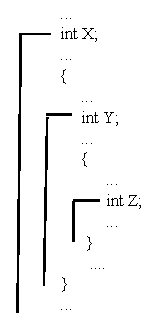
\includegraphics[width=9cm,height=6cm]{images/scope1.eps}}
\setlength{\unitlength}{1cm}
\begin{picture}(12,5.5)
\codefont{
\put(0.2,4.5){int main()\{}
\put(0.5,4.0){int x = 7;}
\put(0.5,3.5){int y;}
\put(0.5,3.0){y = foo(x);}
\put(0.5,2.5){...}
%\put(0.5,2.0){\\ x may have changed}
\put(0.2,1.0){\}}
}
%\put(4.1,3.6){\vector(1,0){5.5}}
\put(4.2,4.8){The box for \codefont{x} is \emph{shared} with the }
\put(4.0,4.3){function \codefont{foo()} under the new name \codefont{z}.}

\put(6.6,3.4){7}
\put(6.4,3.9){\codefont{x}}

\put(3.6,2.4){12}
\put(3.4,2.9){\codefont{y}}

\put(0,0){\large\textbf{main() and its variables}}
% ----------------  func
\codefont{
\put(11.5,4.5){int foo(int \&z)\{}
\put(11.8,4.0){int a;}
\put(11.8,3.5){a = z + 5;}
\put(11.8,3.0){...}
\put(11.8,1.5){return a;}
\put(11.5,1.0){\}}
}

\put(4.4,2.3){The \emph{value} of \codefont{a} is copied into \codefont{y}}
\put(4.4,1.8){when the function returns.}

\put(6.9,3.9){\codefont{z}}

\put(10.1,2.4){12}
\put(9.9,2.9){\codefont{a}}
\put(10.5,0){\large{\textbf{foo() and its variables}}}

\ifcolor\color{\mycolor}{
\put(9.8,2.7){\vector(-1,0){5.5}}
\put(13.35,5.38){\vector(1,-1){0.5}}
\put(3.5,2.3){\line(1,0){0.5}}
\put(3.5,2.8){\line(1,0){0.5}}
\put(3.5,2.3){\line(0,1){0.5}}
\put(4.0,2.3){\line(0,1){0.5}}
\put(10,2.3){\line(1,0){0.5}}
\put(10,2.8){\line(1,0){0.5}}
\put(10,2.3){\line(0,1){0.5}}
\put(10.5,2.3){\line(0,1){0.5}}

\put(6.5,3.3){\line(1,0){0.5}}
\put(6.5,3.8){\line(1,0){0.5}}
\put(6.5,3.3){\line(0,1){0.5}}
\put(7.0,3.3){\line(0,1){0.5}}
\ifcolor}

\end{picture}
\caption{When a function parameter is \emph{pass-by-value}, denoted by the \& symbol in the function's parameter declaration, the variable's ``box'' is ``shared'' between the functions.  Any changes to the parameter's value in the function ``persist'' in the calling function.  Returned values are still copied as normal.  Contrast this to the illustration of pass-by-value in Figure~\ref{fig:arguments} in Chapter 4.}
\label{fig:passbyrefarguments}
\end{figure}

\subsection{Arrays}\index{arrays}

In programming, it's often useful to store many values of the same type.  For example, a list of grades, telephone numbers, baseball scores, etc.  The simplest method to store a list of data is to use an array -- a set of data items, all of the same type, stored sequentially in memory.  
Figure~\ref{fig:array1} illustrates this idea.

Arrays are declared and accessed using square brackets: [ and ].  The general form of an array \emph{declaration} is:\\
\codefont{type name[\emph{N}];}\\
where \codefont{type} is the type of data to be stored, \codefont{int}, \codefont{string}, class, etc.; \codefont{name} is the name of the array; and \codefont{\emph{N}} is the size of the array (i.e., the number of elements the array can hold).  For example, the command:\\
\cf{double values[10];}\\
creates an array that can hold 10 values of type \cf{double}.


The elements of an array are numbered starting from 0.  So, in an array of \codefont{\emph{N}} elements, the elements are numbered from $0$ to \codefont{\emph{N}-1}.  

The general form of a statement to access an array element is:\\
\codefont{\emph{name}[\emph{index}]}\\
where \codefont{\emph{name}} is the name of the array and \codefont{\emph{index}} is the number of the particular item in the array that needs to be accessed.  For example, the command:\\
\codefont{values[3] = 7.7;}\\
sets the \emph{fourth} item in the array called \codefont{numbers} to the value 7.7 and the command:\\
\cf{cout << values[2];}\\
prints the \emph{third} element of the array (because arrays start with element 0).   The index used to access an element of an array can be an integer, an expression, or an integer variable.

Array elements can be accessed \emph{only} one at a time.  For example, copying one array into another requires a loop that copies each element individually; printing an array requires printing each element individually.  

\subsection{Array Bounds}\index{arrays!bounds}

\begin{wrapfigure}{R}{0.5\textwidth} \framebox[\linewidth][l]{\parbox{0.95\linewidth}{\codefont{Out of Bounds Errors and Security} \\
Out of bounds errors are often exploited by hackers to break into programs.  Consider a program that asks the user for a password and stores it in an array.  If the program is not well written, a clever hacker can enter a long password that exceeds the size of the array.  Doing this causes some of the password characters to be written into other parts of memory.  If the over-sized password is carefully designed, some of the characters in the password may be written into, and thereby change, the variable that determines whether the password is correct.  This tricks the program into thinking that a valid password was entered and allows the hacker entrance into the system.  Modern, well-designed systems avoid this problem by only reading as many characters as they can safely store, regardless of how many characters the user actually enters.
}}
\vspace{-0.5cm}
\end{wrapfigure}

When an array is declared in C++, the program sets aside enough contiguous memory to hold the whole array and uses the array name as a pointer to the beginning of the block of memory.  For example, if a program declares an array of 100 integers called \codefont{data}, then the program sets aside enough memory to hold 100 integers and the variable \codefont{data} points to the first element in the array.\footnote{The variable literally stores a number corresponding to the \emph{memory address} where the first element of the array is stored.  Pointers and memory addresses are covered in more detail in the next chapter.}

To access an element of an array, a program starts at the first element of the array and then jumps to the memory location indicated by the index.  For example, the command:\\
\codefont{data[7]}\\
tells the program to start at the location in memory that \codefont{data} points to and then jump forward in memory by seven integers' worth of memory (assuming \codefont{data} is an array of integers) and grabs whatever data is found in that memory location.\footnote{This is why arrays start counting from 0, the array name points to the first element of the array, so a size 0 jump reaches the first element.}

The critical idea is that a C++ program does \emph{not} check whether the place it jumps to is actually within the array.  From the compiler's point of view, it is perfectly acceptable to create an array of 10 elements and then try to access the $11^{th}$ element, or the $1,000^{th}$ element, or even the $-10^{th}$ element.  Trying to access an array element that is not within the range of the array elements is commonly known as an \emph{out of bounds}\index{out-of-bounds}\index{errors!out-of-bounds} error.

%\begin{wrapfigure}{R}{0.5\textwidth} \framebox[\linewidth][l]{\parbox{0.95\linewidth}{\codefont{Creating Libraries} \\
%All of the projects in this text are entered as a single, long program.  More commonly programs are broken up into the main program file and separate libraries.  In the case of the Generic Game program it would be common to put the square class in a separate library.  Generally, this requires putting the code into a separate file and `including' it as an additional library.  However, depending on the programming environment the actual steps may vary, Visual Studio has a specific `add a class' menu option whereas using a command line compiler requires creating the files.  To avoid having to detail multiple approaches all programs are treated as a single file in this text, but you are encouraged to figure out how to break them into separate libraries in your particular programming environment.
%}}
%\vspace{-0.5cm}
%\end{wrapfigure}

Out of bounds errors generally have one of two effects on a program.  If the program tries to access a piece of memory that is too far out of an array, it may end up trying to access a region of memory that the program does not have access to, in which case the operating system forces the program to stop running.\footnote{When a program starts running, the operating system assigns the program its own region of memory to work in; the program is not allowed to go outside this region to keep it from interfering with any other programs.}  Typically, the program crashes and the operating system prints a ``segmentation fault'' message, meaning that the program has stepped outside its allowed segment of memory.  


\begin{figure}
%\centerline{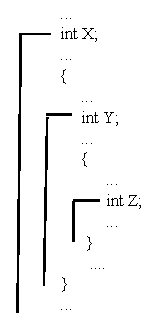
\includegraphics[width=9cm,height=6cm]{images/scope1.eps}}
\setlength{\unitlength}{1cm}
\begin{picture}(12,3.5)
\linethickness{0.3mm}

\put(6,2.8){\codefont{numbers[0]} \hspace{0.4cm}5}
\put(6,2.3){\codefont{numbers[1]} \hspace{0.4cm}6}
\put(6,1.8){\codefont{numbers[2]} \hspace{0.4cm}99}

\put(6,1.3){\codefont{numbers[3]} \hspace{0.4cm}2}

\put(7,0.8){... \hspace{0.8cm} ...}
\put(6,0.25){\codefont{numbers[9]} \hspace{0.4cm}8}

\put(11.3,2.8){\cf{numbers}}

\color{\mycolor}{
\put(8,0.7){\line(1,0){1}}
\put(8,1.2){\line(1,0){1}}
\put(8,1.7){\line(1,0){1}}
\put(8,2.2){\line(1,0){1}}
\put(8,2.7){\line(1,0){1}}
\put(8,0.2){\line(1,0){1}}
\put(8.0,3.18){\line(1,0){1}}
\put(8,3.18){\line(0,-1){3}}
\put(9,3.18){\line(0,-1){3}}

\put(10,3.1){\line(1,0){1}}
\put(10,2.6){\line(1,0){1}}
\put(10,2.6){\line(0,1){0.5}}
\put(11,2.6){\line(0,1){0.5}}
\put(10.3,2.9){\vector(-1,0){1.1}}

}
\end{picture}
\caption{An array of 10 integers.  The array's name is \codefont{numbers}.  The first four values in the array are 5, 6, 99, and 2, the last value is 8.  Note that the array elements are numbered 0 to 9, \emph{not} 1 to 10.  The variable \cf{numbers} (no brackets) keeps track of the beginning of the array.}
\label{fig:array1}
\end{figure}

A more subtle problem arises if a program attempts to access an element that is out of the bounds of an array, but within the region of memory that the program is allowed to use.  Because the access is within the program's memory, the operating system doesn't interfere and the command is allowed to execute.  However, because the access is out of the array's bounds,  a region of memory outside of the array is affected.  For example, consider the following command:\\
\codefont{data[11] = 7;}\\
when data is an array with only 10 elements.  This command starts at \codefont{data[0]}, jumps 11 integers' worth of memory, and places a 7 in that memory location.  However, that memory location is outside the array and is probably being used to store data for a different variable \emph{whose value will be changed.}  Thus, when there is an out of bounds error, a seemingly random variable can have its value changed unexpectedly.  This leads to errors that are unpredictable and very hard to find and fix.  When using arrays, it is critical that all attempts to access array elements are within bounds.

\subsection{Passing Arrays to Functions}

\begin{figure}
%\centerline{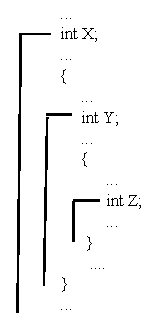
\includegraphics[width=9cm,height=6cm]{images/scope1.eps}}
\setlength{\unitlength}{1cm}
\begin{picture}(12,5.5)
\codefont{
\put(0.2,4.5){int main()\{}
\put(0.5,4.0){int numbers[10];}
\put(0.5,3.5){numbers[0] = 0;}
\put(0.5,3){numbers[1] = 1;}
\put(0.5,2.5){...}
\put(0.5,2.0){foo(numbers);}
\put(0.5,1.5){...}
\put(0.2,1.0){\}}
}
%\put(4.1,3.6){\vector(1,0){5.5}}
%\put(4.2,4.8){The box for \codefont{x} is \emph{shared} with}
%\put(4.2,4.2){\codefont{z} when the function is called.}
\put(5.8,4.3){\codefont{\large\textbf{numbers \hspace*{0.5cm}z}}}
\put(5,3.8){\codefont{numbers[0]} \hspace{0.4cm}1 \hspace{0.34cm}\codefont{z[0]}}
\put(5,3.3){\codefont{numbers[1]} \hspace{0.4cm}2 \hspace{0.34cm}\codefont{z[1]}}
\put(5,2.8){\codefont{numbers[2]} \hspace{0.4cm}88 \hspace{0.18cm}\codefont{z[2]}}
\put(5,2.3){\codefont{numbers[3]} \hspace{0.4cm}4 \hspace{0.34cm}\codefont{z[3]}}
\put(6,1.8){... \hspace{0.8cm} ...}
\put(5,1.25){\codefont{numbers[9]} \hspace{0.4cm}9 \hspace{0.34cm}\codefont{z[9]}}

\put(4.2,2.75){\codefont{.}}
\put(4.2,2.55){\codefont{.}}
\put(4.2,2.35){\codefont{.}}

\put(0,0){\large\textbf{main() and its variables}}
% ----------------  func
\codefont{
\put(11.0,4.5){int foo(int z[])\{}
%\put(11.8,4.0){int a;}
%\put(11.8,3.5){a = z + 5;}
\put(11.5,4.0){...}
\put(11.5,3.5){z[2] = 88;}
\put(11.5,3.0){...}
%\put(11.8,1.5){return a;}
\put(11.0,1.0){\}}
}
\put(10.5,0){\large{\textbf{foo() and its variables}}}

\color{\mycolor}{
\put(7.0,4.18){\line(1,0){1}}
\put(7,3.7){\line(1,0){1}}
\put(7,3.2){\line(1,0){1}}
\put(7,2.7){\line(1,0){1}}
\put(7,2.2){\line(1,0){1}}
\put(7,1.7){\line(1,0){1}}
\put(7,1.2){\line(1,0){1}}

\put(11.3,3.5){\vector(-4,-1){2.1}}
\put(13.25,5.38){\vector(1,-1){0.5}}
\put(3.7,3.55){\vector(4,1){1.2}}
\put(3.7,3.05){\vector(4,1){1.2}}
\put(8,4.18){\line(0,-1){3}}
\put(7,4.18){\line(0,-1){3}}
}
\end{picture}
\caption{Arrays are always passed to functions via pass-by-reference, so the array is ``shared'' between the two functions.  The array is named \codefont{numbers[]} in \codefont{main()} and named \codefont{z[]} in \codefont{foo()}.  Any changes made in the called function ``persist'' in the calling function. So, in this example \cf{z[2]} becomes $88$ in \cf{main()} after the function is called.}
\label{fig:arrayarguments}
\end{figure}

Arrays can be passed to functions as arguments.  
Square brackets [] denote that a function's parameter is an array.  For example, lines 21 and 1c show the syntax for the function declaration (or prototype) and function definition of the \codefont{read\_board()} function, whose parameter is an array of square objects.  However, when an array is passed to the function, the square brackets are not used.  For example, when the array \codefont{the\_board} is passed to the function \codefont{read\_board()} (line 6b) there are no square brackets on the variable name.

C++ takes an important shortcut in passing an array to a function.  It does \emph{not} copy the whole array into the function; instead, it passes the address of the beginning of the array to the function.  This address \emph{references} the location of the array in memory.  Thus, when an array is passed to a function as an argument, it is passed using \emph{pass-by-reference}.  
Figure~\ref{fig:arrayarguments} illustrates this idea.

As with other pass-by-reference arguments, the result of this approach is that the function has direct access to the original data in the array.  Any changes that the function makes to the array will still exist after the function exits.

Finally, it is important to realize that in general, functions won't ``know'' how large an array is.  To overcome this limitation, the size of an array is often passed to the function as a second argument.  That is, a function is passed both an array and an integer denoting the size of the array.  Alternatively a program may use a \emph{global} variable to define the size of an array.  Global variables (described in detail next) are variables that have global\index{global}\index{variables!global} scope and therefore can be accessed by any function in a program without needing to be passed to the function as an argument.  


\subsection{Globals}
A global is simply a variable or constant that is declared before and outside of any function (including the \codefont{main()} function).
According to the rules of scope, this means that its scope extends throughout the entire program.  The variable can be accessed from within any function -- it is global.  

The most common use for globals is to declare a constant value that should be used throughout a program.  For example, imagine a program for calculating the area of different curved shapes.  The value of $\pi$ used (e.g., 3.141 versus 3.141592) could make an important difference in the calculated answers.  If difference functions in the program used different values of $\pi$ the program might produce confusing or nonsensical results.  Creating a single, global variable that stored the value of $\pi$ to be used everywhere in the program would solve this problem.  Making the variable a constant would keep the value from ever changing.

The key word \cf{const} (short for \emph{const}ant) is used to declare a constant.  Once a constant is created, trying to give it a new value anywhere in the program will cause a compiler error. 

 In the Generic Game program length of the game board (\codefont{board\_length}, declared on line 24) is a global, so any function in the game knows the length of the board.  Not only does this avoid errors, it also makes it simple to change the length of the board, simply by changing the variable's value.

\subsection{Characters}

The \codefont{char}\index{character}\index{char@{\cf{char}}}\index{type!char@{\cf{char}}} type (short for character) holds a single character; for example `a', `b', `6', `]', or `.'.  Characters are denoted by single quotes.  Thus,
\codefont{`a'} represents the \emph{character} a; \codefont{a} represents a \emph{variable} named \cf{a}; and \codefont{``a''} is a \emph{string} containing the single character a.   Characters are stored in memory as integers, with each character represented by its own \emph{ASCII}\index{ASCII} value.\footnote{ASCII stands for American Standard Code for Information Interchange.}  For example, the character \codefont{`a'} has the value 97 and the character \codefont{`\#'} has the value 35.  Nonprinting characters like escape and tab also have ASCII values that allow them to be treated as characters.  Because each character has a unique numeric value, characters can be used as \codefont{case} values in a switch statement.  For example,\\
\codefont{
case `a':\\
}
is legal as part of a switch construct, which makes it simple to create menus with character, rather than numeric, options.

\section{Analysis of the Code}

\mysubsubsection{Lines 1-6: \#includes}

As in the previous programs these are preprocessor commands that include additional libraries.  

\mysubsubsection{Lines 8-18: The \cf{Square} Class Declaration}

Lines 8-18 are the declaration of the \cf{square} class.  The class structure is the same as for the \cf{pet} class in the previous project.  The class consists of data members and member functions.  As is common in classes, the data members are private and the member functions are public.  Thus, the only way to change or use the data within an object of type \cf{square} is to use one of the public member functions.  Each square on the game board is represented by one object of type \cf{square}.  So, for a board with 20 squares, 20 objects of type square will need to be created (this is done by creating an \emph{array} of \cf{square} objects, described below).

Each object of type \cf{square} has three data members:
\begin{tight_enumerate}
\item \codefont{move} - This is an integer that stores the distance that a player moves forward or backward after landing on the square.  For example, if a player lands on a square whose \codefont{move} value is -2, they move backwards 2 squares.  For most squares, \cf{move} is 0; nothing special happens.
\item\codefont{message} - This is a string that stores the message that's printed when a player lands on the square.  For most squares, it is blank; there is no special message.
\item\codefont{symbol} - This is a character that stores the symbol/character that is printed on the screen for the square.  A special square (with a nonzero move and a nonblank message) might be printed on the screen as a `?'.  For most squares, the symbol is a space; there is no special symbol.
\end{tight_enumerate}

There are four member functions that can be applied to each object of type \cf{square}:
\begin{tight_enumerate}
\item \codefont{square()} - This is the constructor.  It's called when a new object of type \cf{square} is created.
\item \codefont{print()} - This function `prints' a square -- that is, it prints some of the data associated with an object of type \cf{square}.
\item \codefont{action()} - This function returns the amount that a player should move forward or backward after landing on a square.
\item \codefont{set()} - This function is used to ``set'' the data of an object of type \cf{square}.  The function takes three arguments, corresponding to a square object's three data members.
\end{tight_enumerate}

\mysubsubsection{Lines 20-22: Function Prototypes}

Lines 20-22 define the prototypes for the three functions that are part of the project.  Notice that the program contains both member functions of the square class (lines 14-17) and general functions that are not associated with any class (lines 20-22).  

\mysubsubsection{Line 24: Global  Constant}\index{constant}\index{global}\index{variables!constant}\index{variables!global}

Line 24 defines a \emph{global}, \emph{constant}: \codefont{board\_length}.  The keyword \codefont{const}\index{const} makes the variable a constant, meaning that the value, once set, cannot be changed anywhere else in the code.  Constants are useful for storing values that shouldn't change, values like $\pi$ or the gravitational constant \emph{g}, or in this case, the length of the game board.

The variable \codefont{board\_length} is a global because it is declared before \cf{main()}.  Following the rules of scope (discussed in Chapter 3), this means that the scope of \codefont{board\_length} extends throughout the entire program, including \codefont{main()}, the other functions, and the class.  

\mysubsubsection{Line 4b: Array Declaration}

Line 4b declares an \emph{array} of variables of type \cf{square}.  The array is named \codefont{the\_board}.  The square brackets make this an array declaration, and the value \codefont{board\_length} within the brackets means that the array is \codefont{board\_length} items long.   So, line 4b creates an array of \codefont{board\_length} objects of type \cf{square}.  This array represents the game board (hence the name \codefont{the\_board}).  The $N^{th}$ square on the board (or the $N^{th}$ element of the array) can be accessed by the statement \codefont{the\_board[N]}, but remember that array elements are numbered starting from 0.

\mysubsubsection{Line 5b: Random Seed}
This sets the random seed to be equal to the current time.  This should result in a unique sequence of rolls each time the game is played.

\mysubsubsection{Lines 6b and 1c-13c: The read\_board() Function}\index{files!read}\index{ifstream@{\cf{ifstream}}}\index{libraries!fstream@{\cf{ifstream}}}\index{fstream@{\cf{fstream}}}

The \codefont{read\_board()} function reads a number of data items out of the file ``game.txt'' and stores them in an array of objects of type \cf{square}.   It sets up the special squares on the board.  

Line 6b simply calls the \codefont{read\_board()} function, which is defined on lines 1c-13c.   The return type for the function is void -- it doesn't return anything.  The parameter of the function is \codefont{square b[]}.  This means that the function should receive an \emph{array} (because of the brackets \cf{[]}) of square objects and will, within the function, name the array \codefont{b}.  

Line 2c creates a new variable named \codefont{infile} of type ifstream.  Line 3c uses the \codefont{open()} member function to open the file \codefont{game.txt}. 

Lines 4c-6c declare variables that will be used within the \codefont{read\_board()} function. 

Lines 7c and 12c define a \codefont{while} loop. The condition for the loop is:
\codefont{!infile.eof()}\\
The command \codefont{infile.eof()} calls the function \codefont{eof()}, which is a member function of the class \codefont{fstream} (note the use of the dot notation for a member function of a class).  The function name, \codefont{eof()}\index{eof@{\cf{eof()}}}\index{files!eof@{\cf{eof()}}}, is short for ``End Of File.''  The function \cf{eof()} returns the Boolean value \codefont{true} if the end of the file is reached and \codefont{false} otherwise.  The ! symbol is the Boolean \emph{NOT}.  Thus, line 7c can be read as:
\emph{while infile is not at the end of the file, execute the code in the loop}.

Lines 8c and 9c read data out of the file called ``game.txt'' that was opened on line 3c, and store the data in local variables.  Lines 8c and 9c use notation similar to that used with \codefont{cin}, except that instead of reading data from the keyboard, the data is read from a file.  

Line 9c calls the \codefont{getline()} function, which is defined in the iostream library.  The function \cf{getline()} is a member function of the \cf{ifstream} class, so the dot notation is used.  The function takes a \emph{source} (in this case the variable \codefont{infile}, which is connected to the file ``game.txt'') and reads a string of characters, stopping when it reaches a newline ($\backslash n$) character.  The string is then stored in the second argument to the \codefont{getline()} function, which, in this case is \codefont{square\_message}.

Line 1d in the Listing~\ref{listing:game.txt} is the first line of the \codefont{game.txt} file.  So, after lines 8c and 9c are executed, the program should store the following:\\
\codefont{square\_number = 7}\\
\codefont{square\_move = -2}\\
\codefont{square\_symbol = `?'}\\
\codefont{square\_message = ``Go back 2 squares.''}\\

Finally, line 10c checks that the \codefont{square\_number} is within the bounds of the array.  If it is, line 11c takes the last three values and passes them to the \codefont{set()} member function of object number \codefont{square\_number} of the array \codefont{b[]}.  Recall that \codefont{b[]} is an array of objects of type \cf{square}.  Thus, in the first part of line 11c: \codefont{b[square\_number]}, refers to one of the objects in this array.  The rest of line 11c, \codefont{.set(square\_move,square\_symbol,square\_message)}, calls the \codefont{set()} function of the class \cf{square} and passes three values in as arguments.  The \codefont{set()} function stores the data it receives in the square object's data members.  

Because all of the data is read from a file, it is not necessary to change \emph{any} of the code to change the board.   The board can be completely changed simply by modifying the file ``game.txt.''

\mysubsubsection{Lines 7b, 8b, 26b, 27b, and 14c-25c: The print\_board() Function}

The \codefont{print\_board()} function prints the game board for one player.  To print the board for both players it gets called twice.  It's called twice on lines 7b and 8b to print the board the first time, and on lines 26b and 27b to print the board after each player's turn.  It prints the board by stepping through each element in the array of squares and either printing the square or, if a player is in the square, prints the player's number.

The \codefont{print\_board()} function is defined starting on line 14c.
The function doesn't return any values, so the return type is \codefont{void}.  It takes three arguments: the first is an array of objects of type \cf{square} (the board), the second is an integer storing the current player's position, and the third is an integer storing the current player's number.

Lines 15c and 20c use a new type of loop, the \codefont{for}\index{for loop@{\cf{for} loop}}\index{loops!for@{\cf{for}}} loop.  A \codefont{for} loop loops for a set number of steps, typically using a counter variable to count how many steps the loop has gone through.  In this case, the loop command is:\\
\codefont{for(int i = 0; i < board\_length; i++)}\\
When the loop is first entered, it executes the \codefont{int i = 0;} command, which creates a new variable \codefont{i} and sets its value to 0.  Next, the loop checks the condition \codefont{i $<$ board\_length}.  If it is true, the code within the loop is executed; if it is false, the loop is skipped (the program jumps to line 21c).  Because \codefont{i} is initially 0 and \codefont{board\_length} is 20 (line 24)  the loop is executed.  When the end of the loop is reached, at line 25c, execution returns to the beginning of the loop and the command \codefont{i++} is executed.  This increases \codefont{i} by 1.  Then the condition is checked again.  If it is still true, the code within the loop is executed again; if it has become false, the loop is skipped.  

\begin{wrapfigure}{R}{0.5\textwidth} \framebox[\linewidth][l]{\parbox{0.95\linewidth}{\codefont{Arrays and \cf{for} Loops} \\
Because arrays generally have to be accessed one element at a time, they are often used in conjunction with \cf{for} loops.  For example, the code\\
\codefont{
for(int i =0; i < array\_length; i++)\\
\hspace*{0.5cm}b[i] = a[i];\\}
will copy the values of array \codefont{a} correctly into array \codefont{b}.  The statement
\codefont{b = a;} will \emph{not} copy the array elements.  

Similarly, to print all of the elements of an array, the code\\
\codefont{
for(int i =0; i < array\_length; i++)\\
\hspace*{0.5cm}cout << a[i] << endl;\\}
will work, but\\
\codefont{cout << a;} will \emph{not} print the array elements.
}}
\vspace{-0.5cm}
\end{wrapfigure}

Thus, in the loop defined on lines 15c and 20c, the loop counter \cf{i} starts at 0, each time through the \codefont{for} loop, \codefont{i} increases by 1 until it is no longer less than \codefont{board\_length}, at which point the loop is exited.  The \codefont{for} loop counts from 0 to the length of the board and either prints what appears in each square on the board (line 17c) or prints the player's number (line 19c).

During each iteration of the loop, the \codefont{if} statement on Line 16c checks whether this is \emph{not} the player's current position (i.e., whether \codefont{i} is not equal to \codefont{player\_position}).  If it is not the player's position, it calls the \codefont{print()} function on object \codefont{b[i]} -- the \emph{i}th element in the array \codefont{b}.  This happens on line 17c:\\
\codefont{b[i].print();}\\
where \codefont{b} is the array of square objects corresponding to the game board, \codefont{i} is the current square on the board (the one being printed), and the \codefont{print()} function is a member function of the \cf{square} class.  So, this command ``asks'' the \emph{i}th square object of the array \codefont{b} to print itself.  (The \codefont{print()} member function of the square class is described below.)

If the current value of \codefont{i} \emph{is} equal to the player's position, then the player's number is printed instead (line 19c).  

Line 21c prints the word ``goal,'' marking the end of the board.

Lines 22c and 23c define a second \cf{for} loop.  This one prints a series of hyphens to denote the middle of the board.  Finally, line 24c adds a last new line to make the output cleaner, and the function returns from the final closing bracket on line 25c.

Note that the \codefont{print\_board()} function is called on both line 7b and line 8b.  The first time it is called, the arguments are \codefont{the\_board}, \codefont{player1\_position}, and the number 1.  So, the function prints the board and places a 1 in player 1's position.  The second time it is called, the arguments are \codefont{the\_board}, \codefont{player2\_position}, and the number 2.  So, the function prints the board and places a 2 in player 2's position.  

\mysubsubsection{Lines 9b-29b: The Game Loop}

Lines 9b and 29b define the main game loop.  It is quite similar to the game loop used for NIM in Chapter 2, except that the condition for continuing the loop is:\\
\codefont{((player1\_position < board\_length - 1) \&\& (player2\_position < board\_length-1))}.\\
The program will continue the loop when: 
\emph{player 1's position is less than the board length-1 AND player 2's position is less than the board length-1}\index{AND@{\cf{AND}}}\index{Boolean!AND@{\cf{AND}}}.
 The symbols, \&\&, define the Boolean AND, which is true only if \emph{both} arguments are true.  So if player 1 hasn't reached the end of the board and player 2 hasn't reached the end of the board, the program will loop, continuing the game. 

The $-1$ is included in the test conditions because the board (being an array) starts at 0.  So, the last square on a twenty square board is square number nineteen. 

%Note that the symbols \&\& stand for the Boolean AND operation.  Also, recall that in an array with $N$ elements the elements are numbered from 0 to $N-1$, so the actual board squares are also numbered from 0 to \codefont{board\_length-1} and so play continues until one of the players reaches the \codefont{board\_length} - 1 square.

\mysubsubsection{Lines 10b-13b: Player Move}
Line 10b is just output telling the current player to press Enter to roll. Line 11b ignores any input, but still waits for the Enter key to be pressed.  Without it (try commenting it out), the game zips by in a flash.  Line 12b generates the player's actual roll, following the same general form as the random move in NIM.  
%In this case the modulus operation (the \% operator) returns a number between 0 and 4 because any random number divided by 5 gives a remainder between 0 and 4 and then adds 1 to it to give a roll between 1 and 5.  Of course, these can be changed to make the rolls in any range the programmer likes.  Finally 
Line 13b prints the roll.  %This is not necessary for the functioning of the program as the player's `piece' is moved automatically, but the player should know what they rolled rather than having to count backwards to figure it out.

\mysubsubsection{Lines 14b-25b: The Move} 

Lines 14b, 20b, 21b, and 25b define an if-else structure used to make sure that the correct player gets to move.  Lines 15b and 21b add the current roll to the current player's position using the \codefont{+=} operator.


\begin{wrapfigure}{R}{0.5\textwidth} \framebox[\linewidth][l]{\parbox{0.95\linewidth}{\codefont{Curly Braces (\{\}'s) or No Curly Braces} \\
In the previous programs, curly braces (\{\}'s) were used to denote blocks of code within if-else statements and loops, but the if-else statement on lines 16c-20c do not use curly braces.  This works because there is only one line of code for the if condition and one line of code for the else condition.  Curly braces are only \emph{required} when the condition applies to more than one line of code.  However, curly braces can always be included, even if they only surround one line of code.  In general, including braces is a good idea,  they are omitted here to save space.  The same rules apply to loops that include only one line of code; for example, lines 22c and 23c.
}}
\vspace{-0.5cm}
\end{wrapfigure}

 Lines 16b and 22b call the \codefont{check\_position()} function.
A lucky (or unlucky) roll or square could send the player beyond the bounds of the board.  So, the \codefont{check\_position()} function is necessary to check whether the player's position is less than 0 (line 27c) or greater than the board length (line 29c), and to correct the player's position if it has exceeded the bounds of the board.
The \codefont{check\_position()} function is called each time a player's position is changed. 
The test conditions are less than 0 or greater than \codefont{board\_length-1} because as an array, the board squares are numbered from 0 to \codefont{board\_length-1}.

The function uses a pass-by-reference parameter.  Instead of returning the new position, the function simply changes the argument's value (line 28c or 30c).  However, because the parameter \codefont{p} is pass-by-reference, as determined by the \& symbol in function declaration (line 22) and the function definition (line 26c), the change made to \codefont{p} in the function changes the \codefont{player1\_position} or \codefont{player2\_position} variable that was passed into the function (lines 16b, 18b, 22b, and 24b).

After the player's roll has been added to their position and his or her position has been checked against the length of the board, and corrected if necessary, the board array is checked to see if anything special happens in the square the player landed in.  This is done on line 17b or line 23b, with the statement:\\
\codefont{player1\_position += the\_board[player1\_position].action();}\\
The \cf{+=} operator is used to change the value of the player's position by the amount \emph{returned} by the function call: \codefont{the\_board[player1\_position].action();}

Then \codefont{the\_board[player1\_position]} is the square object corresponding to the location of the player.  For example, if player 1 is at position (or square) 3, then the variable \codefont{player1\_position} holds the value \codefont{3} and therefore \codefont{the\_board[player1\_position]} refers to square 3.  The next part of the command \codefont{.action()} calls the member function \codefont{action()} for that particular square.  

The \codefont{action()} member function is described in detail next.  For now, it's sufficient to know that it prints the message associated with the square (e.g., ``Bad winds, go back three squares'') and returns the distance the player moves (e.g., -3).  In the initial version of the game most squares have no effect and don't print any message.  

After the player's position has been updated to reflect the action, if any, for the square he or she landed in (line 17b or line 23b), the position is checked again to make sure that the player is still within the bounds of the board.  (This isn't necessary if the programmer is careful with actions; for example, no action sends a player who lands on square 2 back 7 squares.  However, it is good programming practice to have the program double-check because the person rewriting the game file may not understand the details of the game.)  

After the player has been moved by an action, the new square is \emph{not} checked for another action.  So, if a player lands on a square that sends him or her back 3 squares and the new square landed on would send him or her forward 4 squares, the player doesn't go forward 4 squares.  This can be changed, but the current approach avoids the possibility of the player getting caught in an infinite loop of ``go forward 2'' ``go back 2.'' 

\mysubsubsection{Lines 26b-27b: Reprinting the Board}

Lines 26b and 27b simply reprint the board with the new player positions by calling the \codefont{print\_board()} function.

\mysubsubsection{Line 28b: Next Player's Move}

Line 28b changes the current player from 1 to 2 or vice versa, similar to how it was done in NIM.

\mysubsubsection{Lines 30b-33b: The End of the Game}

If the program breaks out of the \cf{do-while} loop on lines 9b-29b, it's because one of the players has reached the end of the board, making the condition on line 29b false.  Line 30b changes the current player \emph{back} to the winner (the current player was changed on line 28b, so the identity of the winner has to be changed back).  Line 31b prints the winner message.  Line 32b pauses and waits for the user to hit Enter.  

\subsection{Lines 33c-49c: The \cf{Square} Class Definitions}

This section details the member functions of the \cf{square} class: \codefont{square()}, \codefont{action()}, \codefont{print()}, and \codefont{set()}.  These are all very short functions, but are useful for keeping the data about the squares of the board separate from the rest of the program.  The text \codefont{square::} in the function definitions indicates that these functions are members of the \cf{square} class and not stand alone functions like \codefont{read\_board()}, \codefont{print\_board()}, and \codefont{check\_position()}.

\mysubsubsection{Lines 33c-37c: The \cf{square()} Function (the constructor)}

The function \codefont{square()} is the constructor for the \cf{square} class.  It is called whenever a new object of type \cf{square} is called.  It sets the initial values of an object of type \cf{square}, setting the \codefont{symbol} to a space (line 34c), the \codefont{move} to 0 (line 35c), and the \codefont{message} to ``'', that is, no message, (line 36c).  These are the default values for ``normal'' squares on the board.

For the special board squares these values are changed by the \codefont{read\_board()} function (lines 1c-13c) calling the \codefont{set()} function (lines 45c-49c, described below).

\mysubsubsection{Lines 38c-41c: The \cf{action()} Function}

The \codefont{action()} function is called when a player lands on a square.  Line 39c prints the message associated with the square (e.g., ``Bad winds, go back 3 squares'' for special squares, or a blank message ``'' for normal squares).  Line 40c returns the amount that the player is forced to move by the square (e.g., -3).  This return value is used to adjust the player's position on line 17b or line 23b, depending on whose turn it is.

\mysubsubsection{Lines 42c-44c: The \cf{print()} Function}

The \codefont{print()} member function prints the symbol associated with a square; for example, a blank for normal squares and a special symbol like `?' or `*' for special squares.  The function is called by the \codefont{print\_board()} function.

\mysubsubsection{Lines 45c-49c: The \cf{set()} Function}

The \codefont{set()} member function is used to set the data that a square object holds.  When a new square is created, the constructor sets all of its data to the default values: no action, no message, and a space for a symbol.  The \codefont{set()} member function is used by the \codefont{read\_board()} function to change these values for special squares (line 11c).

\subsection{The Data File}

Listing~\ref{listing:game.txt} is the data file, called ``game.txt'' and used to define the board.  The data file is opened and read by the \codefont{read\_board()} function.  This function expects to find very specific data in a very specific order:
\begin{tight_itemize}
\item An integer - This is the number of the special square to be added to the board. It should be between 0 and \codefont{board\_length-1}.
\item A character - This is the symbol to be printed on the board for the special square.
\item An integer - This is the amount a player is moved if he or she lands on the square (negative numbers for backward moves).
\item A string - This is the message to be printed if the player lands on the special square.
\end{tight_itemize}
For example, line 1d in the file is:\\
\codefont{7 -2 ? Go back 2 squares.}\\
which means square number 7 is special (this is actually the eighth square because the array starts  at zero).  It is printed on the board with a ?.  If a player lands on it, the message ``Go back 3 squares'' is printed, and they go back 2 squares (-2).  

The \emph{mechanics} of the game are defined by the program: how many players there are, who moves when, what the rolls are, etc.  However, the details of the game (which squares are special, what effects they have, and what messages are printed) are defined by the data file.  A completely different flavor of game, with different special squares and different messages, can be created simply by rewriting the data file ``game.txt'' without changing any of the code.  

\vspace{+0.25cm}
{\color{\mycolor}\noindent\hrulefill}
\section{Exercises: Modifying the Program}

The current game is very simple and not particularly interesting to play.  Changing the output and the game file would make the game more interesting.  In addition, there are ways to change the game to make it more of a challenge to the players.  

\mysubsubsection{Exercise 1: Customize the Game}
Rewrite the ``game.txt'' file to customize the game.  First, pick a theme: a sailing game, a car racing game, an ``escape the zombies'' game, a ``kill all humans'' game, etc..  Then change the ``game.txt'' file, particularly the messages, to fit the theme.  Add more lines to the data file to make more squares on the board special.  It's a good idea to test each addition or change to the game file individually.  It's very frustrating to add 15 new lines and then have to figure out which of the new lines contains the typo that keeps the file from being read correctly.

\mysubsubsection{Exercise 2: Add an Introduction}
Add an introduction to the game that sets the stage and explains the rules.  For example, if your game is a zombie apocalypse game, add an introduction describing how the zombie's arose and the players' goals.    \\
{\bf Challenge:} Add the introduction to the beginning of the ``game.txt'' file and have the program read and print it.  This is important if you want the same program to be able to read and play different game files.

\mysubsubsection{Exercise 3: Improve the Output}
Change how many blank lines are added between moves to make it clearer how the players are moving along the board.  Then change the \codefont{print\_board()} function to vary how the board itself is drawn.  Add vertical bars ($|$'s)  between each square to make the board look more like a series of separate squares, or add a row of hyphens above the board.

\mysubsubsection{Exercise 4: Players' ``Pieces''}
Currently the players appear on the board as a 1 and a 2.  Change the game so that they appear as different characters and to allow each player to pick his or her own symbol.  This will require some extra code at the beginning of the game asking the player what symbol is wanted and two new variables of type \codefont{char} to store those symbols.

\mysubsubsection{Exercise 5: Other changes}
There are a lot of other simple changes that can be made to the game.  Change the length of the board.   Notice how much harder it would be to change the length of the board if instead of the global constant \codefont{board\_length}, the actual number 20 (or 19) was used everywhere.  It would be necessary to find and change every instance of the value, instead of just making one change to the constant.  Then change the range of allowed rolls.  Try changing the game so that negative rolls are possible; for example, players can roll any value from -1 to 4. 

\mysubsubsection{Exercise 6:  Multi-player}
Change the game so three or more players can play.  Then change the game so that the user can decide how many players there will be (up to some limit).  There needs to be a new variable to keep track of the total number of players.  The value of the variable should be set by the user at the beginning of a game.  Then this value is used as part of the modulus operation on lines 28b and 30b to decide who goes next.  To print the board, it will probably be necessary to add a \cf{for} loop that loops over the number of players, calling \codefont{print\_board()} once for each player.  Finally, the if-else statement on lines 14b-25b probably needs to be replaced with a switch statement based on the \codefont{current\_player}.

\section{Problems}
The potential for modifying the generic game should now be clear.  There are also more complicated changes that can be made to the overall game mechanics.
\begin{enumerate}[{\bf 1.}]

\item {\bf Many games in one}\\
 Currently, the program always reads the game data from the file ``game.txt,'' which means the program always plays the same game.  Have the program ask the user (e.g., in the \codefont{read\_board()} function), which file to open (or which game to play) and then open the appropriate file.  This will allow the user to choose between games (e.g., sailing or escape the zombies), when the program starts.

\item {\bf Random squares}\\
 Instead of always moving the same number of squares, make special squares move the player by a random amount.  The \cf{action()} function will need to be changed to generate a random action instead of always returning the same value.  
In addition, the ``game.txt'' file, the \codefont{read\_board()} function, and the \cf{square} class will need to be rewritten so that there is a way to indicate and remember whether a special square should be a random square or a deterministic square.  One approach is to use two integers in the ``game.txt'' file to set the upper and lower limits of a random move.  If the two bounds are the same (e.g., -3 and -3), then the move is deterministic.

\item {\bf More complex squares}\\
 Add a type of square that has a more complex effect.  For example, a square that allows the player to take another roll or squares that force the player to miss a turn.  As in the previous problem this will probably require changing the ``game.txt'' file, the \codefont{read\_board()} function, and the \cf{square} class so that the new square types can be correctly read from the data file and stored in the square objects.

\item {\bf Additional game variables}\\
 Have players start with some gold (or health or fame, etc.).  As the game progresses, special squares cause each player's gold (or health, etc.) to increase and decrease.  Change the victory conditions to match the new variable.  For example, the game might end when the first player reached the goal, but the winner is the player with the most gold (and maybe the first player to reach the goal gets some bonus gold making it more likely that the player will win).  Make sure that the game's introduction, instructions, and comments accurately explain the new version.

\item {\bf Player choices}\\
One limitation of the game is that it's completely random; there's no element of skill.  Fix this by giving the players' options.  Allow players to choose between moving two squares ahead (slow, but sure) or rolling to move a random amount (say from 1 to 4).  Which choice is more strategic would depend on what squares are ahead (does the player want to try to jump over an unlucky square?) and how far ahead or behind he or she (a player who was already way ahead might take the slow, but steady option, whereas a lagging player might hope to get lucky and catch up).

\item {\bf Squares with choices}\\
Create a new type of square that gives the player an option.  For example, a square where the player who lands on it either goes back three squares OR gives the opponent a +1 bonus on his or her next roll.  This requires a more complex ``game.txt'' file to denote these special squares and both the ability to read the file and store the information in the \cf{square} class.\\
{\bf Challenge:} Invent at least two more types of special squares that give the player an option and include them in your game. In some cases both options could be beneficial.   Possible options for a player to choose from could include, going backwards $N$ squares, losing a turn, sending an opponent forwards, getting an extra roll, getting a bonus on the next roll, etc.

\end{enumerate}